\let\negmedspace\undefined
\let\negthickspace\undefined
\documentclass[journal]{IEEEtran}
\usepackage[a5paper, margin=10mm, onecolumn]{geometry}
%\usepackage{lmodern} % Ensure lmodern is loaded for pdflatex
\usepackage{tfrupee} % Include tfrupee package

\setlength{\headheight}{1cm} % Set the height of the header box
\setlength{\headsep}{0mm}     % Set the distance between the header box and the top of the text

\usepackage{gvv-book}
\usepackage{gvv}
\usepackage{cite}
\usepackage{amsmath,amssymb,amsfonts,amsthm}
\usepackage{algorithmic}
\usepackage{graphicx}
\usepackage{textcomp}
\usepackage{xcolor}
\usepackage{txfonts}
\usepackage{listings}
\usepackage{enumitem}
\usepackage{mathtools}
\usepackage{gensymb}
\usepackage{comment}
\usepackage[breaklinks=true]{hyperref}
\usepackage{tkz-euclide} 
\usepackage{listings}
% \usepackage{gvv}                                        
\def\inputGnumericTable{}                                 
\usepackage[latin1]{inputenc}                                
\usepackage{color}                                            
\usepackage{array}                                            
\usepackage{longtable}                                       
\usepackage{calc}                                             
\usepackage{multirow}                                         
\usepackage{hhline}                                           
\usepackage{ifthen}                                           
\usepackage{lscape}
\begin{document}
\bibliographystyle{IEEEtran}
\title{4.13.7}
\author{EE25BTECH11002 - Achat Parth Kalpesh }
{\let\newpage\relax\maketitle}
\renewcommand{\thefigure}{\theenumi}
\renewcommand{\thetable}{\theenumi}
\setlength{\intextsep}{10pt} % Space between text and floats
\numberwithin{equation}{enumi}
\numberwithin{figure}{enumi}
\renewcommand{\thetable}{\theenumi}
\parindent 0px



\textbf{Question:}\\
If $a,b$ and $c$ are in A.P, then the straight line $ax +by +c=0$ will always pass through a fixed point whose coordinates are \rule{1cm}{0.01pt}.

\textbf{Solution:}\\
Let the equation $ax +by +c=0$ be represented as
\begin{align}
\label{eq:0.1}
    \vec{n}^\top \vec{x} = -c\\
    \vec{n} = \myvec{a\\b}
\end{align}
Let $\vec{p}$ be the fixed point.\\
The condition that $a,b,c$ are in arithmetic progression is
\begin{align}
    2b=a+c \quad\Longrightarrow\quad  a - 2b = -c,
    \label{eq:0.3}
\end{align}
Thereby,
\begin{align}
  \myvec{a\\b}^\top \myvec{1\\-2} = -c
\end{align}
Comparing it with \eqref{eq:0.1} we get
\begin{align}
    \vec{p} = \myvec{1\\-2}
\end{align}
\begin{figure}[h]
    \centering
    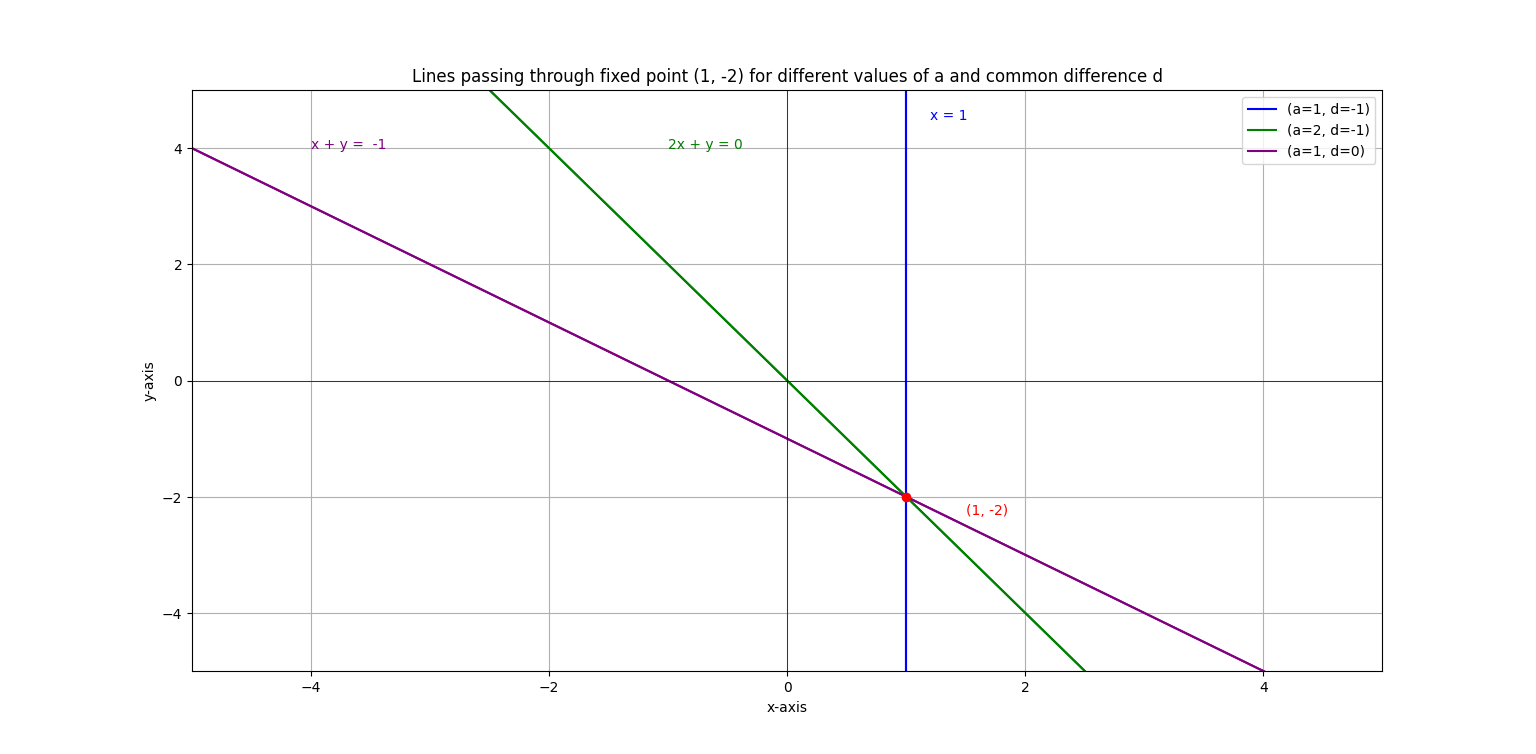
\includegraphics[width=0.9\columnwidth]{figs/figure_py.png}
    \caption{Graph}
    \label{fig:fig}
 \end{figure}
\end{document}